%%%%%%%%%%%%%%%%%%%%%%%%%%%%%%%%%%%%%%%%%%%%%%%%%%%%%%%%%%%%%%%%%%%%%%%%%%%%%%
\documentclass[aspectratio=169]{beamer}            % Generate slides
%\documentclass[handout]{beamer}   % Generate handouts (6 slides to 1 page)
%\documentclass[aspectratio=169]{beamer}  % Use widescreen 16:9 aspect ratio
    % Possible aspect ratios are 16:9, 16:10, 14:9, 5:4, 4:3 (default) and 3:2
    % (Remember to remove the colon)

\usetheme{UoB}
%\usetheme[compress]{UoB}     % Compress the margins
%\usetheme[nourl]{UoB}        % Remove the footer with the URL
%\usetheme[nowatermark]{UoB}  % Remove the watermark from the title page

% Generate handouts with notes (3 slides + 3 notes to 1 page)
%\mode<handout>{
%  \pgfpagesuselayout{3 on 1 with notes}[a4paper,border shrink=10mm]
%}

\usepackage{nomencl} % nomenclature generation via makeindex
	\makenomenclature
\usepackage{tikz}
\usetikzlibrary{matrix,chains,scopes,arrows,positioning,fit,
	decorations.pathmorphing,decorations.markings,shapes,calc}
\usepackage[binary-units = true]{siunitx}
\usepackage{subfig}

\everymath{\displaystyle}

\graphicspath{{./Figures/}}

%%%%%%%%%%%%%%%%%%%%%%%%%%%%%%%%%%%%%%%%%%%%%%%%%%%%%%%%%%%%%%%%%%%%%%%%%%%%%%
\title[Bio-Inspired Distributed Sensing]{Bio-Inspired Distributed Sensing for
	Improved Flight Control}
%\subtitle{Subtitle}
\author{Sergio A. Araujo-Estrada}
\institute{Research Associate \\
	Aerospace Engineering Department \\
	\href{mailto:s.araujoestrada@bristol.ac.uk}{s.araujoestrada@bristol.ac.uk}}
\date{Thursday, May 3}

%%%%%%%%%%%%%%%%%%%%%%%%%%%%%%%%%%%%%%%%%%%%%%%%%%%%%%%%%%%%%%%%%%%%%%%%%%%%%%
\begin{document}

\titlepage

%%%%%%%%%%%%%%%%%%%%%%%%%%%%%%%%%%%%%%%%%%%%%%%%%%%%%%%%%%%%%%%%%%%%%%%%%%%%%%
\begin{frame}{Overview}
	\tableofcontents
\end{frame}

%%%%%%%%%%%%%%%%%%%%%%%%%%%%%%%%%%%%%%%%%%%%%%%%%%%%%%%%%%%%
\section{Introduction}
\subsection{Motivation}
\begin{frame}{Motivation}
  
  \begin{columns}
    \begin{column}{0.5\textwidth}
      \begin{itemize}
	\item<1->{Current UAV autopilot technologies}
	\item<3->{Challenges}
	\item<5->{Potential use of force and flow information}
      \end{itemize}
    \end{column}
    \begin{column}{0.5\textwidth}  %%<--- here
      \only<2>{
	\begin{itemize}
	  \item[-]Inertial
	  \item[-]Single point air speed
	  \item[-]GPS
	  \item[-]Vision
	\end{itemize}
      }
      \only<4>{
	\begin{itemize}
	  \item[-]Intrinsic nonlinear dynamics
	  \item[-]Classic control strategies limitations
	  \item[-]Limitations of inertial controls
	\end{itemize}	  
      }
      \only<6>{
	\begin{itemize}
	  \item[-]Gust alleviation
	  \item[-]Aeroelastic effects
	  \item[-]Additional 'hidden' information
	\end{itemize}
      }
    \end{column}
  \end{columns}
  
\end{frame}

%%%%%%%%%%%%%%%%%%%%%%%%%%%%%%%%%%%%%%%%%%%%%%%%%%%%%%%%%%%%
\subsection{Previous Research}
\begin{frame}{Previous Research}

  \begin{columns}
    \begin{column}{0.4\textwidth}
      \begin{itemize}
	\item<2->Strain sensing
	\item<4->Pressure sensing
      \end{itemize}
    \end{column}
    \begin{column}{0.6\textwidth}
      \only<2>{
	\begin{figure}[!htb]
	  \centering
	  \includegraphics[height=0.45\textwidth]{EasySkyGlider_WTGustTest.eps}
	  \caption{Strain sensing platform}
	  \label{Fig:ExpPlatform}
	\end{figure}
      }
      \only<3>{
	\begin{figure}[!htb]
	  \centering
	  % StrainSensorsInWing.tex
\resizebox{!}{0.45\textwidth}{
	\begin{tikzpicture}
		% Auxiliary objects definition
		\tikzstyle{LabelObject}=[fill=white,rectangle,rounded corners,line width=0.5mm,%
			align=center]
		\tikzstyle{ArrowObject}=[red,line width=0.5mm, -latex]
		% Graphics display
	  \node[anchor=south west,inner sep=0] (image) at (0,0)%
	  {\includegraphics[width=\textwidth,trim= 50mm 0mm 50mm 0mm,clip,angle=180]%
	  	{StrainSensorsInWing.eps}};
	  % Define scope with 'image' dimensions as reference
	  \begin{scope}[x={(image.south east)},y={(image.north west)}]
%			  	\draw[help lines,xstep=.05,ystep=.05] (0,0) grid (1,1);
%			  	\foreach \x in {0,1,...,9} { \node [anchor=north] at (\x/10,0) {0.\x}; }
%			    \foreach \y in {0,1,...,9} { \node [anchor=east] at (0,\y/10) {0.\y}; }
	    %% Auxiliary coordinates
	    \coordinate (L0) at (0.875,0.41);   \coordinate (R0) at (0.050,0.42);
	    \coordinate (L1) at (0.800,0.42);   \coordinate (R1) at (0.125,0.41);
	    \coordinate (L2) at (0.720,0.41);   \coordinate (R2) at (0.200,0.42);
	    \coordinate (L3) at (0.640,0.42);   \coordinate (R3) at (0.280,0.41);
	    \coordinate (L4) at (0.565,0.41);   \coordinate (R4) at (0.360,0.42);
	    \coordinate (L5) at (0.490,0.42);   \coordinate (R5) at (0.440,0.41);
	    %% Labels
	    \draw(0.875,0.25) node[LabelObject] (L0_Label) {${L0}$};
	    \draw(0.800,0.55) node[LabelObject] (L1_Label) {${L1}$};
	    \draw(0.720,0.25) node[LabelObject] (L2_Label) {${L2}$};
	    \draw(0.640,0.55) node[LabelObject] (L3_Label) {${L3}$};
	    \draw(0.565,0.25) node[LabelObject] (L4_Label) {${L4}$};
	    \draw(0.490,0.55) node[LabelObject] (L5_Label) {${L5}$};
	    \draw(0.440,0.25) node[LabelObject] (R5_Label) {${R5}$};
	    \draw(0.360,0.55) node[LabelObject] (R4_Label) {${R4}$};
	    \draw(0.280,0.25) node[LabelObject] (R3_Label) {${R3}$};
	    \draw(0.200,0.55) node[LabelObject] (R2_Label) {${R2}$};
	    \draw(0.125,0.25) node[LabelObject] (R1_Label) {${R1}$};
	    \draw(0.050,0.55) node[LabelObject] (R0_Label) {${R0}$};
	    %% Arrows
			\draw[ArrowObject] (L0_Label.north) -- (L0);
			\draw[ArrowObject] (L1_Label.south) -- (L1);
			\draw[ArrowObject] (L2_Label.north) -- (L2);
			\draw[ArrowObject] (L3_Label.south) -- (L3);
			\draw[ArrowObject] (L4_Label.north) -- (L4);
			\draw[ArrowObject] (L5_Label.south) -- (L5);
			\draw[ArrowObject] (R5_Label.north) -- (R5);
			\draw[ArrowObject] (R4_Label.south) -- (R4);
			\draw[ArrowObject] (R3_Label.north) -- (R3);
			\draw[ArrowObject] (R2_Label.south) -- (R2);
			\draw[ArrowObject] (R1_Label.north) -- (R1);
			\draw[ArrowObject] (R0_Label.south) -- (R0);
	  \end{scope}
	\end{tikzpicture}
}
	  \caption{Strain sensing platform instrumentation}
	  \label{Fig:ExpPlatformInst}
	\end{figure}
      }
      \only<4>{
	\begin{figure}[!htb]
	  \centering
	  \includegraphics[height=0.45\textwidth]{Bixler_WTTest.eps}
	  \caption{Pressure sensing platform}
	  \label{Fig:ExpPlatform}
	\end{figure}
      }
      \only<5>{
	\begin{figure}[!htb]
	  \centering
	  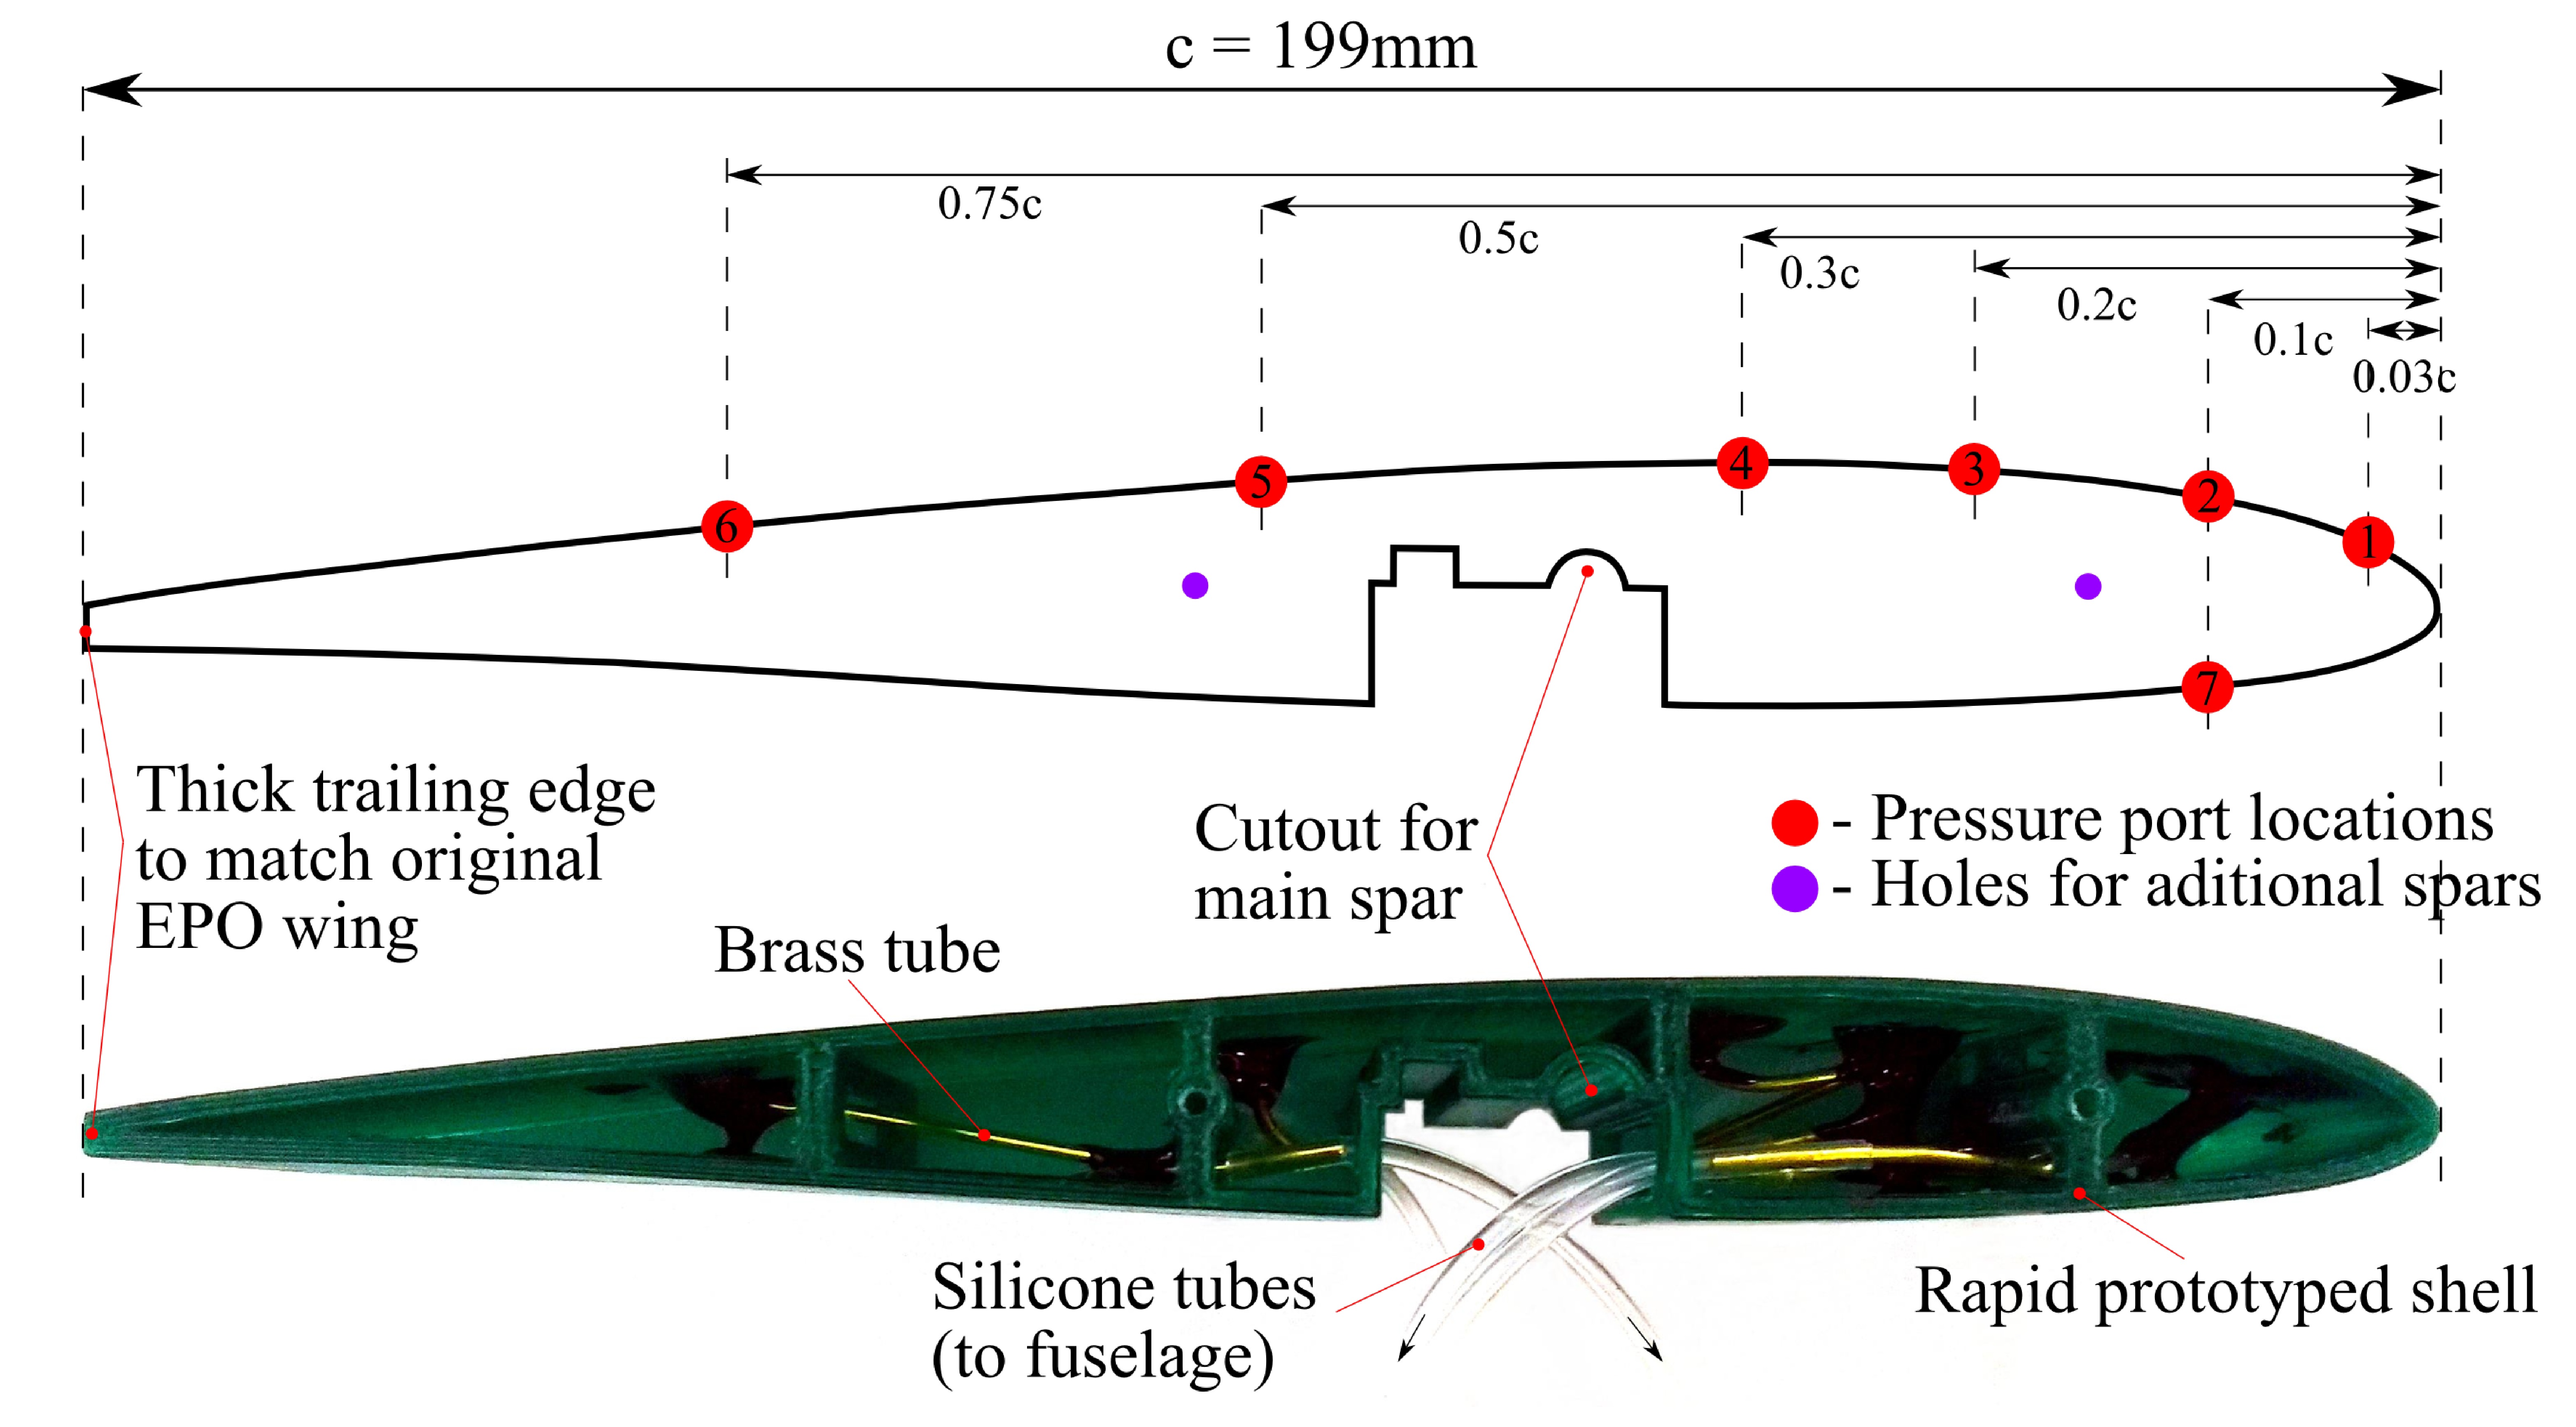
\includegraphics[height=0.45\textwidth]{wingInsertDiagram.eps}
	  \caption{Pressure sensing platform instrumentation}
	  \label{Fig:ExpPlatform}
	\end{figure}
      }
    \end{column}
  \end{columns}
  
%   \begin{block}{A block}
%     What was the goal of your previous research?
%     What/How did we found it? and anyone who might have helped you!.
%   \end{block}

\end{frame}

%%%%%%%%%%%%%%%%%%%%%%%%%%%%%%%%%%%%%%%%%%%%%%%%%%%%%%%%%%%%
\subsection{Research Problem}
\begin{frame}{Research Problem}
  Use force and flow sensing to improve performance of UAVs flight control systems.\\
  \pause
  To achieve this:
  \begin{itemize}
    \item<3-> Develop distributed force and flow sensing system for a small scale fixed wing UAV
    \item<4-> Integrate force and flow sensing into conventional flight control system architecture
    \item<5-> Measure response of systems to controlled and natural turbulence
    \item<6-> Develop advanced reflexive flight control system
  \end{itemize}
\end{frame}

%%%%%%%%%%%%%%%%%%%%%%%%%%%%%%%%%%%%%%%%%%%%%%%%%%%%%%%%%%%%
\begin{frame}{}

  Research divided into two phases:
  \begin{columns}
    \begin{column}{0.5\textwidth}
      \vspace{-0.5cm}
      \begin{itemize}
	\item<2->Wind tunnel experiments using WT model
	\item<3->Outdoors experiments using flying platform
      \end{itemize}
    \end{column}
    \begin{column}{0.5\textwidth}
      \begin{itemize}
	\item<4->[-]Build and instrument a WT model with a distributed array of pressure and strain sensors
	\item<4->[-]Carry out calibration \& characterisation (WT, indoor and outdoor)
	\item<4->[-]Design and implement closed loop control algorithms that use information from distributed array
      \end{itemize} 
    \end{column}
  \end{columns}
  
\end{frame}

%%%%%%%%%%%%%%%%%%%%%%%%%%%%%%%%%%%%%%%%%%%%%%%%%%%%%%%%%%%%
\begin{frame}{The hypothesis (or prediction)}
  What do you think will happen?
  
  Fit strain \& differential pressure sensors
  Carry out WT experiments
  Carry out outdoors experiments
  
  \begin{itemize}
    \item AoA, Windspeed aero loads compuation/prediction/estimation
    \item Characterisation of pressure, strain \& force signals as function of ${\alpha}$, V
      \& ${\delta_{ail}}$
    \item Acquisition of training/testing daat sets for ANN for ${\alpha}$, V \&
      ${\delta_{ail}}$ prediction
    \item Identification of stall characteristic markers in pressure \& strain signals, e.g.
      frequency, variance
    \item Acquisition of pressure \& strain characteristic response to change in ${q}$
    \item Explore pressure \& strain response to conditions similar to perching manoeuvre\
    \item Emulation of pressure \& strain response to gusts
    \item Identify pressure \& strain response to varying ${q}$, i.e. ${\dot{q}}$
    \item Vibration of wing has been observed during and after stall. How does this affect
      pressure \& strain signals?
    \item Identify pressure \& strain response to varying ${\delta_{ail}}$, i.e.
      ${\dot{\delta}_{ail}}$
  \end{itemize}
\end{frame}

%%%%%%%%%%%%%%%%%%%%%%%%%%%%%%%%%%%%%%%%%%%%%%%%%%%%%%%%%%%%
\section{Experiment}
\subsection[Setup]{Setup}
\begin{frame}{Experimental Setup}
  A wing model was instrumented with a distributed array of sensors. The main characteristics of the instrumentation are as follows:
  \begin{itemize}
    \item{chord-wise array of 30 pressure ports in two sections along the span}
    \item{span-wise array with 16 strain gauges}
    \item{data acquisition system using MCU, sampling \@ \SI{100}{\hertz}}
    \item{1-DOF pitch motion wind tunnel rig}
    \item{servo system for automated motion}
  \end{itemize}
\end{frame}

%%%%%%%%%%%%%%%%%%%%%%%%%%%%%%%%%%%%%%%%%%%%%%%%%%%%%%%%%%%%
\begin{frame}[plain]
  \begin{figure}[!htb]
    \centering
    % WingSensorDescription.tex

\tikzstyle{RectObject1}=[rectangle,draw=blue,rounded corners,line width=1.0mm,minimum width=3.0em,%
	minimum height=16.5em]
\tikzstyle{RectObject2}=[rectangle,draw=blue,rounded corners,line width=1.0mm,minimum width=2em,%
	minimum height=2em]
\tikzstyle{LabelObject}=[fill=white,rectangle,rounded corners,line width=0.5mm,%
	align=center]
\tikzstyle{ArrowObject}=[red,line width=1.0mm, -latex]

\resizebox{!}{0.45\textwidth}{
	\begin{tikzpicture}
		\node[anchor=south west,inner sep=0] (image) at (0,0)%
			%{\includegraphics[width=\textwidth]{WingSensorDescription.eps}};
			{\includegraphics[width=\textwidth]{WingInstrumentation.eps}};
		% Define scope with 'image' dimensions as reference
		\begin{scope}[x={(image.south east)},y={(image.north west)}]
			%\draw[help lines,xstep=.05,ystep=.05] (0,0) grid (1,1);
			%\foreach \x in {0,1,...,9} { \node [anchor=north] at (\x/10,0) {0.\x}; }
			%\foreach \y in {0,1,...,9} { \node [anchor=east] at (0,\y/10) {0.\y}; }
			\pause
			
			% Pressure Elements
			\draw(0.330,0.475) node[RectObject1] (PressSensSecA) {};
			\draw(0.730,0.475) node[RectObject1] (PressSensSecB) {};
			% Pressure Labels
			\draw(0.54,0.2) node[LabelObject] (PressSensSecA_Label) {Pressure Port\\Inserts};
			% Pressure Arrows
			\draw[ArrowObject] (PressSensSecA_Label.north west) -- (PressSensSecA.east);
			\draw[ArrowObject] (PressSensSecA_Label.north east) -- (PressSensSecB.west);
			\pause
			
			% Strain Elements
			\draw(0.240,0.580) node[RectObject2] (StrainSens01) {};
			\draw(0.425,0.580) node[RectObject2] (StrainSens02) {};
			\draw(0.630,0.580) node[RectObject2] (StrainSens03) {};
			\draw(0.820,0.580) node[RectObject2] (StrainSens04) {};
			% Strain Labels
			\draw(0.54,0.9125) node[LabelObject] (StrainSens01_Label) {Strain Gauge\\Arrays};
			% Strain Arrows
			\draw[ArrowObject] (StrainSens01_Label.west) -- (StrainSens01.north east);
			\draw[ArrowObject] (StrainSens01_Label.south west) -- (StrainSens02.north);
			\draw[ArrowObject] (StrainSens01_Label.south east) -- (StrainSens03.north);
			\draw[ArrowObject] (StrainSens01_Label.east) -- (StrainSens04.north west);
			\pause
		\end{scope}
	\end{tikzpicture}
}
    \caption{Wing model experimental platform}
    \label{Fig:ExpPlatform}
  \end{figure}
\end{frame}

%%%%%%%%%%%%%%%%%%%%%%%%%%%%%%%%%%%%%%%%%%%%%%%%%%%%%%%%%%%%
\subsection[Preliminary Results]{Preliminary Results}
\begin{frame}[plain]{Preliminary Results}
  Record the information you get from your experiment.
	
  \begin{figure}[!htb]
    \centering
    \subfloat[Chord-wise Normalised Pressure\label{fig:ExpPlatform_Pressure}]{%
	    \includegraphics[width=0.4\textwidth]{PressureCoeffDistribution.eps}}\qquad
    \subfloat[Span-wise Normalised Bending Moment\label{fig:CharSignals_Bending}]{%
	    \includegraphics[width=0.4\textwidth]{BendingMomentDistribution.eps}}
    \caption{Characteristic signals from distributed sensing array}
    \label{Fig:CharSignals}
  \end{figure}

\end{frame}

%%%%%%%%%%%%%%%%%%%%%%%%%%%%%%%%%%%%%%%%%%%%%%%%%%%%%%%%%%%%
\begin{frame}{My discoveries}
  What did you learn after testing?
  \begin{itemize}[<+->]
    \item These will get revealed one by one
      \begin{itemize}
	\item Indented bullets
	\item Some more indented bullets
      \end{itemize}
    \item Another bullet point
    \item Yet another bullet point
  \end{itemize}
\end{frame}

%%%%%%%%%%%%%%%%%%%%%%%%%%%%%%%%%%%%%%%%%%%%%%%%%%%%%%%%%%%%
\begin{frame}[plain]
  This is the most important takeaway that everyone has to remember.
\end{frame}

%%%%%%%%%%%%%%%%%%%%%%%%%%%%%%%%%%%%%%%%%%%%%%%%%%%%%%%%%%%%
\section{Conclusions}
\begin{frame}{Conclusions}
  What is the conclusion of your experiment?
  Did the results support your hypothesis or predicted outcome?
  How will your findings help the area of science you’ve researched?
\end{frame}

%%%%%%%%%%%%%%%%%%%%%%%%%%%%%%%%%%%%%%%%%%%%%%%%%%%%%%%%%%%%
\section{Further Work}
\begin{frame}{Further Work}

  What will you do with your findings next?
  How will you further your research/findings?

  Wind tunnel testing platform
  -Design and implement closed loop control algorithms
  -Carry out closed loop wind tunnel experiments
  
  Flying platform
  -Wind tunnel experiments
  -Outdoors flight tests
  
\end{frame}

%%%%%%%%%%%%%%%%%%%%%%%%%%%%%%%%%%%%%%%%%%%%%%%%%%%%%%%%%%%%
\end{document}

%%%%%%%%%%%%%%%%%%%%%%%%%%%%%%%%%%%%%%%%%%%%%%%%%%%%%%%%%%%%%%%%%%%%%%%%%%%%%%
